% ----------------------------------------------------------------------

\newpage

\subsection{\bb Test}
\label{ss:bb}

\subsubsection{Purpose}

The \bb test is meant to flag any problems with the bump bonds that connect the sensor to the ROCs
and form the path for the charge generated in the silicon sensor to be recorded by the ROCs.
This test takes advantage of a parallel route designed for the calibration signal in the ROC.
This route can be seen at the top left of Figure~\ref{fig:puc}, 
connecting the source of the \vcal calibration pulse to the ``top metal pad'' 
by closing the switch labeled ``sensor calib'' instead of the standard ``calib'' switch.
The ``top metal pad'' is located near the edge of the \roc on the side facing the sensor.
The calibration pulse can pass via capacitive coupling from this pad, 
across the \roc-sensor air gap, and into the silicon sensor.
The calibration pulse then makes its way back into the \roc via the bump bond and can be read out as normal.
Using this signal path that contains the bump bond, 
the presence of the bump and the quality of the electrical connection it establishes between the sensor and the \roc can be tested.

Currently in pXar there are four variants of bump bonding tests,
optimized for different bump bonding processes (and bump ball sizes).  
For FPix modules, the standard test is the {\tt BB3} test.
This document focuses on this specific \bb test version.

\subsubsection{Methodology}

The \bb test is essentially an \scurves test with respect to \vthrcomp, 
with the calibration signal routed through the sensor instead of directly to the readout electronics.
\vcal is configurable and by default is set to 250 (high range).
In any case, \vcal should be set quite high since a large signal loss is expected going through the air gap from \roc to sensor.
The number of triggers used is also configurable (default is 5).
From the \vthrcomp s-curve for each pixel, the turn on value is extracted, 
defined as the value of \vthrcomp for which the efficiency surpasses 50\%.
For pixels with good bump bonds, these thresholds should be distributed normally, i.e.~as a Gaussian curve.
The distribution of the \vthrcomp turn-on is fitted to a Gaussian, the mean and width of which are recorded.
In this fit, peaks near 0 or 255 are excluded, since these most likely come from dead pixels.
Since variations in the mean of this turn-on are observed in odd and even columns, 
this fitting is done separately for the odd/even columns in the \roc.
Pixels that turn on at much higher than average \vthrcomp values have higher than average signal loss.
Leveraging this fact, pixels with turn-on values more than $5\times\sigma$ above the mean are flagged as bad.

\subsubsection{Output}

Output from the \bb test is shown in Figures~\ref{fig:bb3_thr_calSMap_VthrComp}-\ref{fig:bb3_dist_rescaledThr}.
Figure~\ref{fig:bb3_thr_calSMap_VthrComp} shows a \roc map of the raw turn-on values extracted from the \vthrcomp s-curve for each pixel.
Figures~\ref{fig:bb3_dist_thr_calSMap_VthrComp_EvenCol} and \ref{fig:bb3_dist_thr_calSMap_VthrComp_OddCol} 
show the 1D distributions of the even and odd columns in Figure~\ref{fig:bb3_thr_calSMap_VthrComp}, 
along with their best-fit curves and arrows located $5\times\sigma$ above the mean of the curve.
The means of these distributions are noticeably different, which is why these two distributions are fit separately.
These distributions are then recombined, but since they have different means and widths,
it does not make sense to combine them directly.
Instead, each entry is scaled to represent the number of standard deviations it is away from the mean.
We refer to this scaled value as the fit ``residual''.
Figures~\ref{fig:bb3_rescaledThr} and \ref{fig:bb3_dist_rescaledThr} show a 2D \roc map and a 1D distribution of these fit residuals, respectively.
Any pixels above the black arrow in Figure~\ref{fig:bb3_dist_rescaledThr} are flagged as anomalous bumps.

\begin{figure}[!htp]
\centering
\begin{minipage}{0.45\textwidth}
  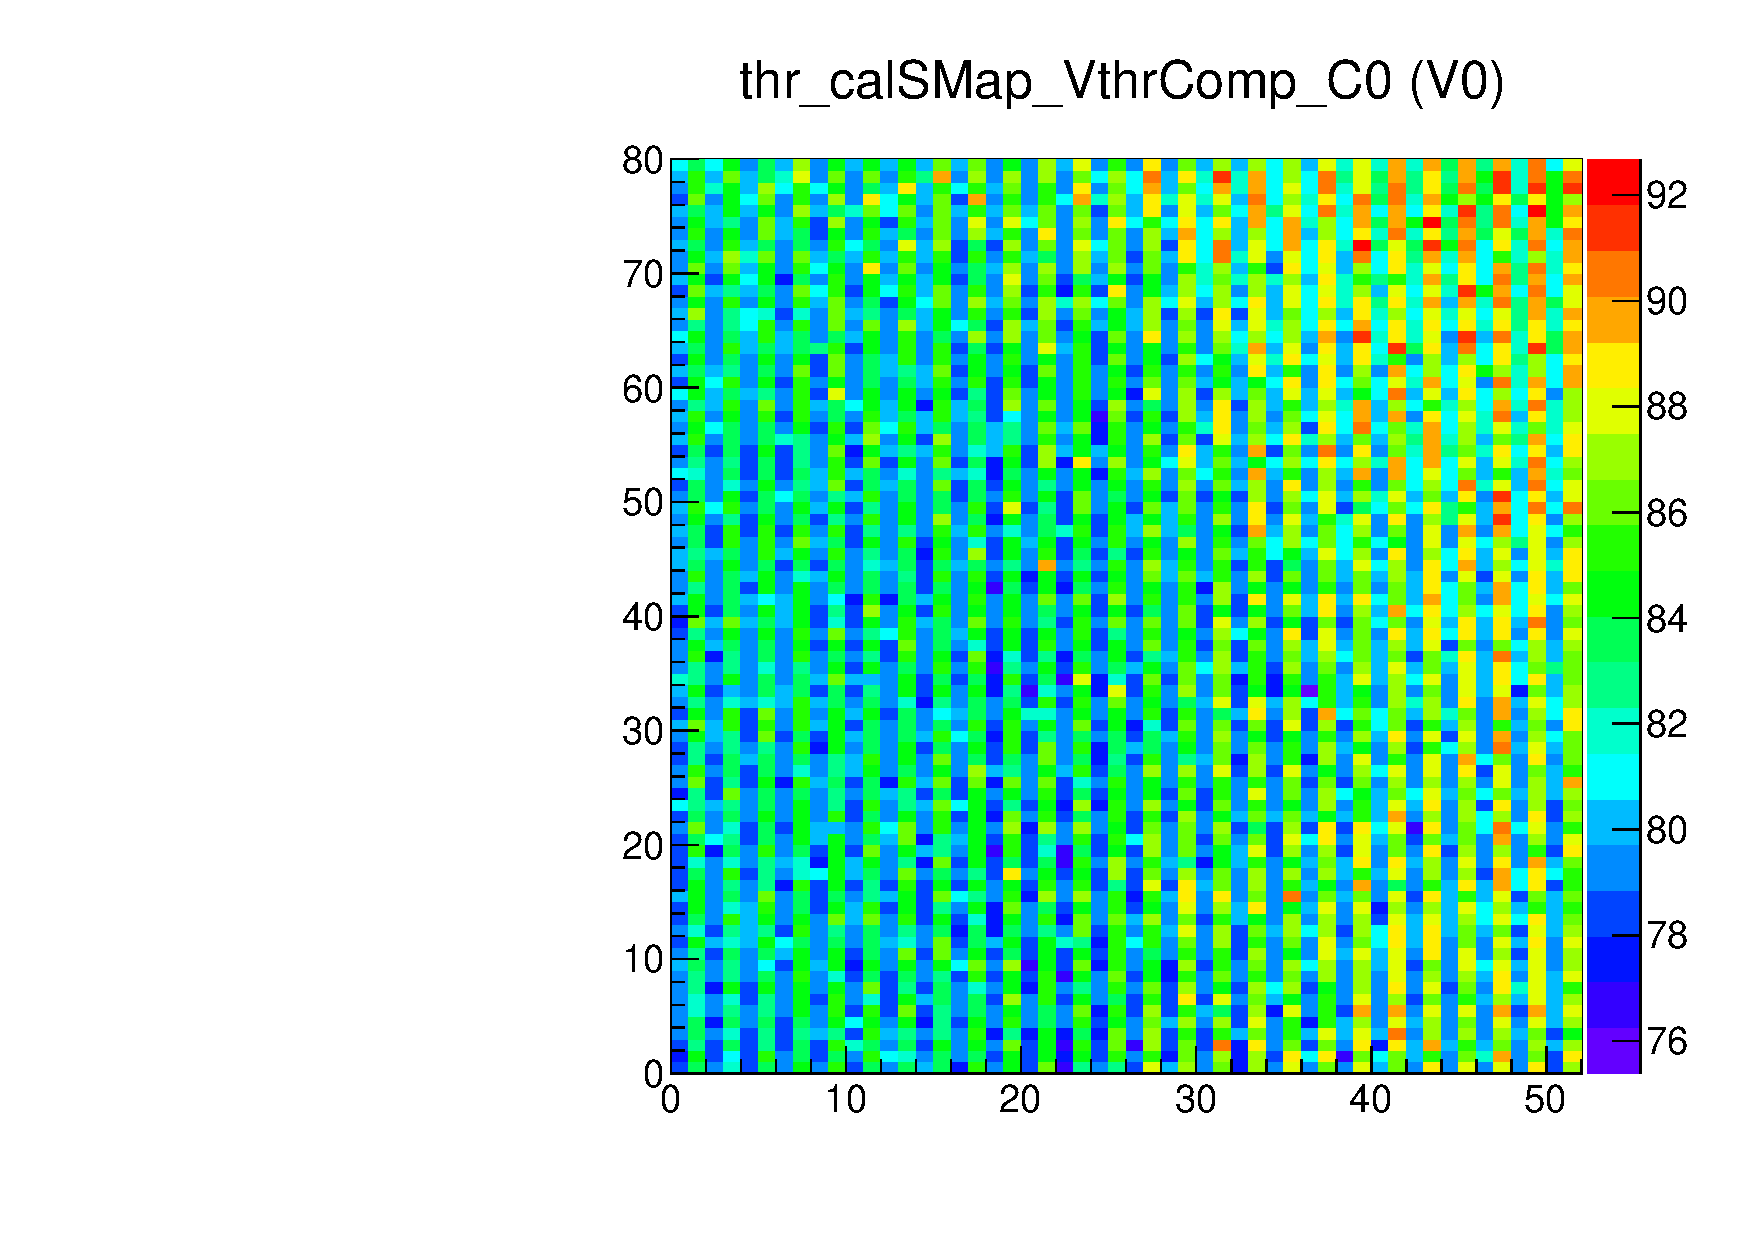
\includegraphics[width=1.0\textwidth]{figures/bb3_thr_calSMap_VthrComp.pdf}
  \caption{\roc map of the raw \vthrcomp turn-on values when passing the calibration pulse through the sensor.}
  \label{fig:bb3_thr_calSMap_VthrComp}
\end{minipage}
\end{figure}

\begin{figure}[!htp]
\centering
\begin{minipage}{0.45\textwidth}
  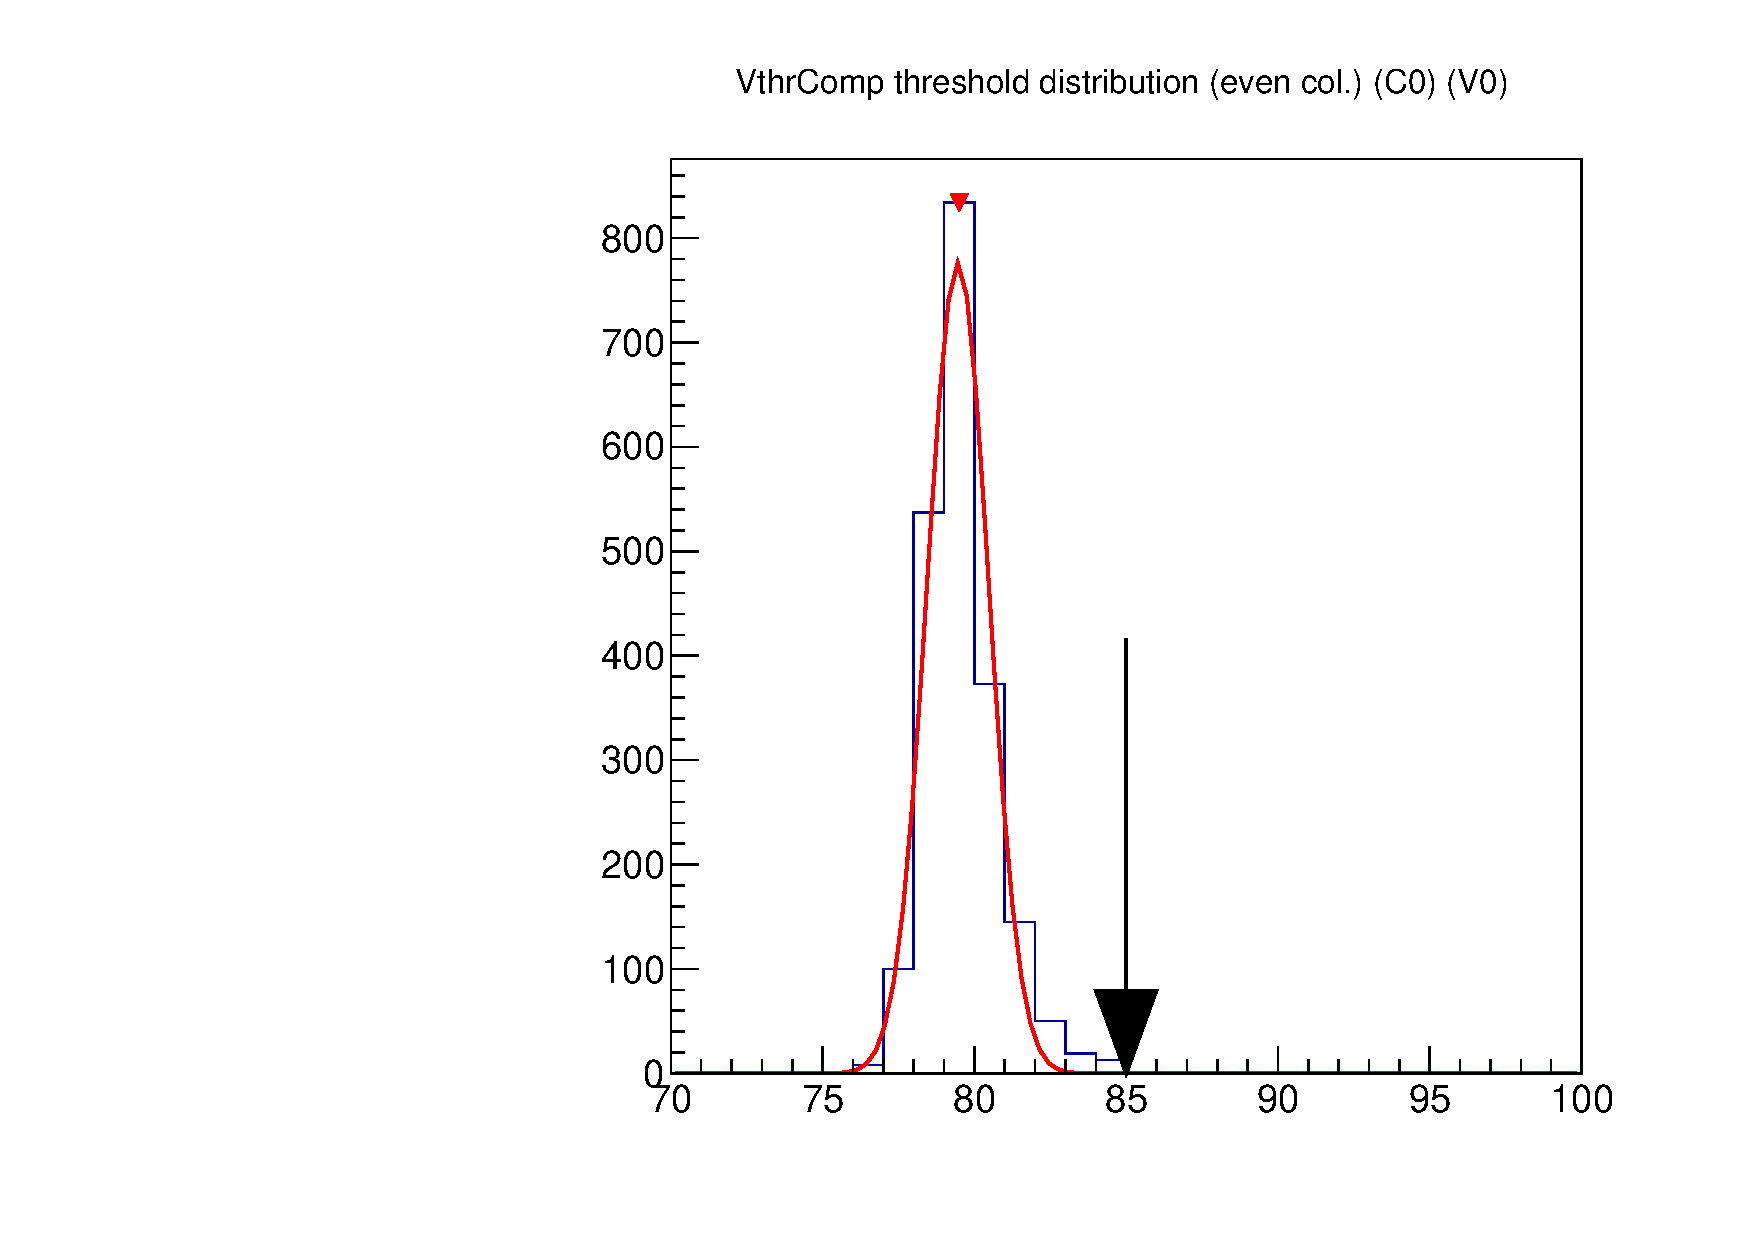
\includegraphics[width=1.0\textwidth]{figures/bb3_dist_thr_calSMap_VthrComp_EvenCol.pdf}
  \caption{1D distribution of the even columns in Figure~\ref{fig:bb3_thr_calSMap_VthrComp}.
  The red curve is a Gaussian fit to the data.
  The black arrow corresponds to 5$\sigma$ above the fitted peak.
  [original range 0-255]}
  \label{fig:bb3_dist_thr_calSMap_VthrComp_EvenCol}
\end{minipage}
\hspace{0.3cm}
\begin{minipage}{0.45\textwidth}
  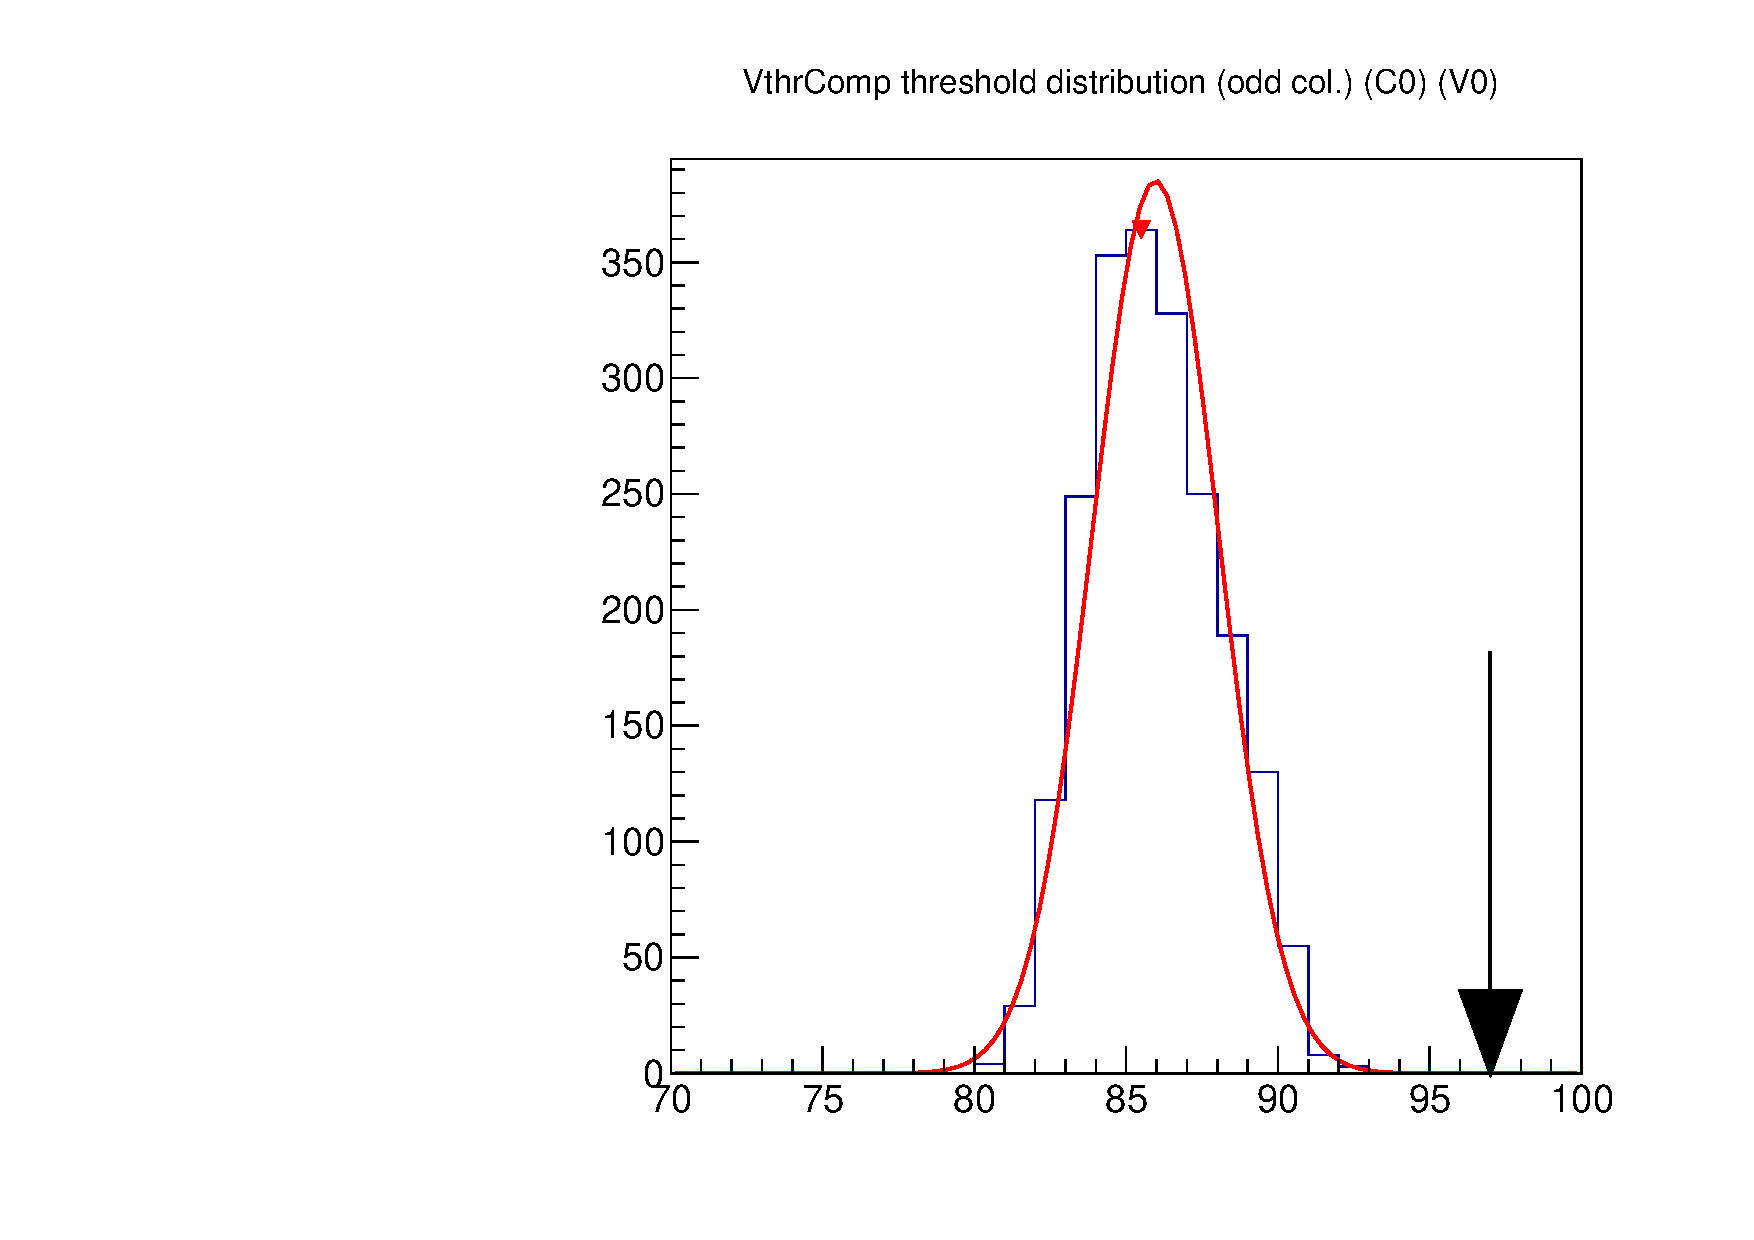
\includegraphics[width=1.0\textwidth]{figures/bb3_dist_thr_calSMap_VthrComp_OddCol.pdf}
  \caption{1D distribution of the odd columns in Figure~\ref{fig:bb3_thr_calSMap_VthrComp}.
  The red curve is a Gaussian fit to the data.
  The black arrow corresponds to 5$\sigma$ above the fitted peak.
  [original range 0-255]}
  \label{fig:bb3_dist_thr_calSMap_VthrComp_OddCol}
\end{minipage}
\end{figure}

\begin{figure}[!htp]
\centering
\begin{minipage}{0.45\textwidth}
  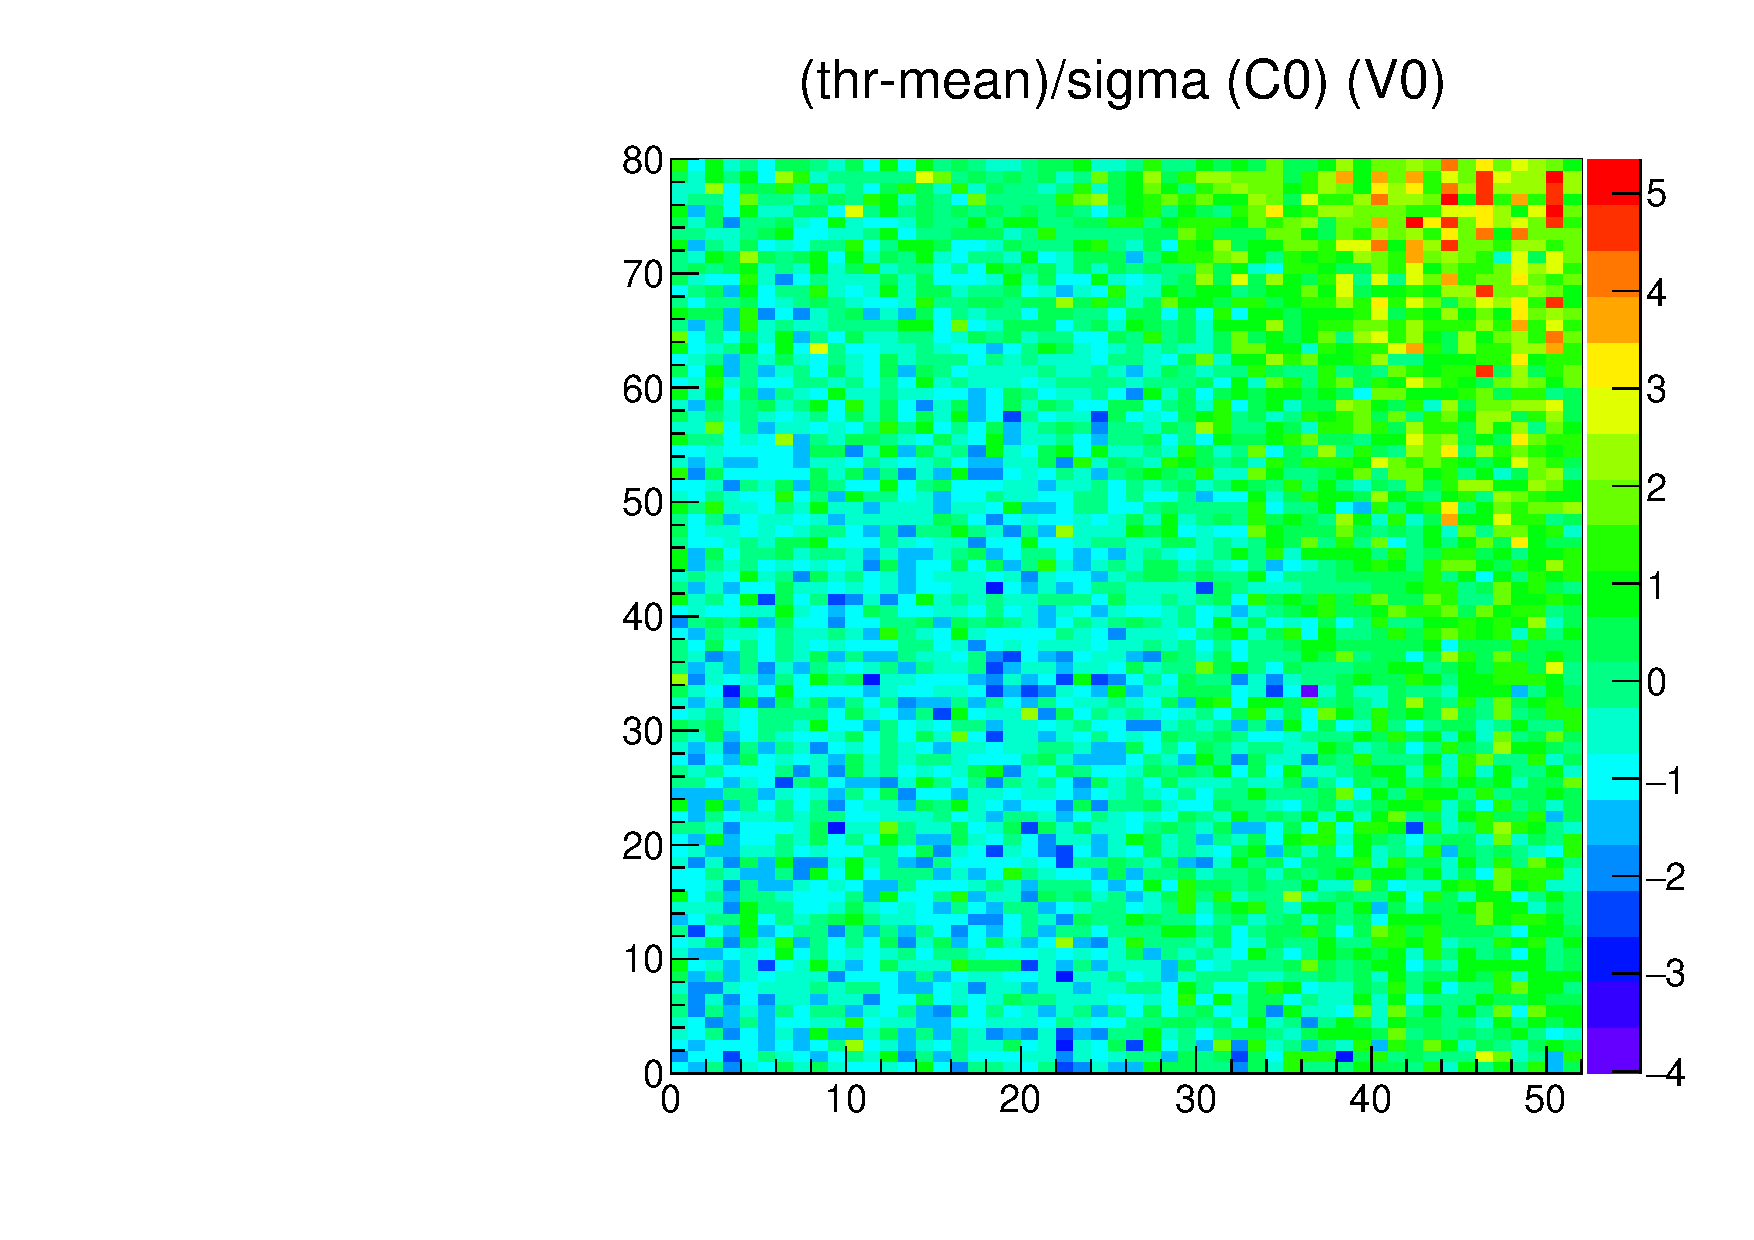
\includegraphics[width=1.0\textwidth]{figures/bb3_rescaledThr.pdf}
  \caption{\roc map of the residuals of the \vthrcomp turn-on values, 
  calculated separately for even and odd columns.}
  \label{fig:bb3_rescaledThr}
\end{minipage}
\hspace{0.3cm}
\begin{minipage}{0.45\textwidth}
  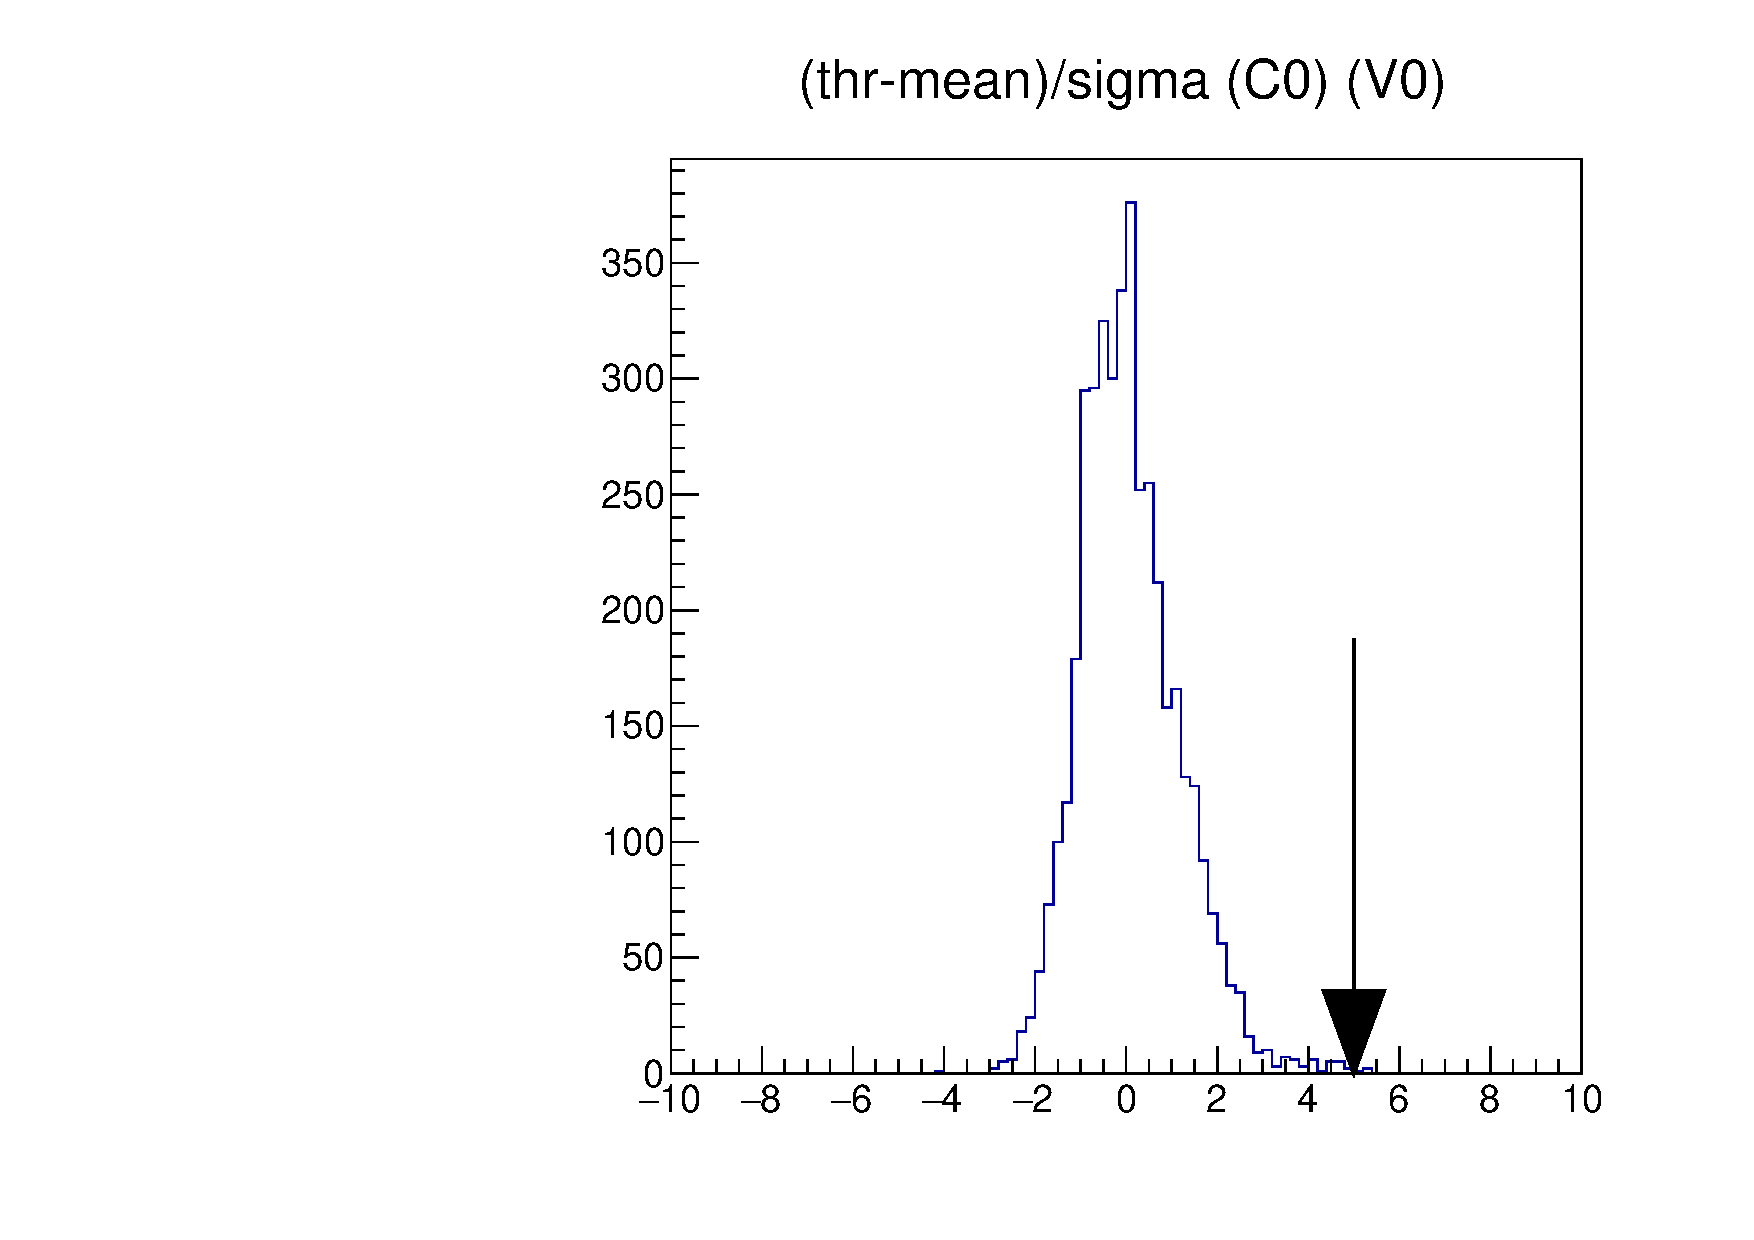
\includegraphics[width=1.0\textwidth]{figures/bb3_dist_rescaledThr.pdf}
  \caption{1D distribution of \roc map in Figure~\ref{fig:bb3_rescaledThr}.
  Pixels with turn-on values more than 5$\sigma$ above the \roc mean 
  (marked by the black arrow) are flagged as faulty.
  The first (last) bin of the plot contains the underflow (overflow) entries.}
  \label{fig:bb3_dist_rescaledThr}
\end{minipage}
\end{figure}

